% Shared content of the SHORT PlantIQ paper. Edit THIS file; short.tex (two columns) and short_onecol.tex (one column)
% both \input it, so the two PDFs always have identical content. The full-length paper is paper_content.tex.
\IEEEoverridecommandlockouts
\usepackage{cite}
\usepackage{amsmath,amssymb,amsfonts}
\usepackage{graphicx}
\usepackage{textcomp}
\usepackage[T1]{fontenc}
\usepackage{newtxtext} % Times text, as in the IEEE template output
\usepackage{xcolor}
\usepackage{booktabs}
\usepackage{makecell}
\usepackage{array}
\usepackage{url}
\usepackage{tikz}
\providecommand{\plantiqfigw}{\columnwidth}
\usetikzlibrary{arrows.meta,positioning,fit,backgrounds,calc}

\newcommand{\yes}{\checkmark}
\newcommand{\no}{$\times$}
\newcommand{\part}{$\sim$}

\tikzset{
  box/.style={draw=black!70, rounded corners=2pt, align=center, font=\scriptsize, inner sep=3pt, fill=white},
  mod/.style={box, fill=blue!6, minimum width=2.6cm, minimum height=1.0cm},
  ext/.style={box, fill=black!4, dashed},
  arr/.style={-{Stealth[length=4pt]}, black!75, line width=0.5pt},
  grp/.style={draw=black!35, rounded corners=3pt, inner sep=5pt},
  grplabel/.style={font=\scriptsize\bfseries, black!70},
}

\begin{document}

% Registered first so that the coffee CNN paper is [1] and the coffee RAG paper is [2].
\nocite{anudeep2024cnn,selvakumar2024rag}

\title{PlantIQ: A Multimodal, Retrieval-Grounded Decision-Support Platform for Smallholder Coffee Growers in Karnataka}

% #2 is added after "and Engineering" (e.g. the AI & ML specialisation); the department is split over two lines so
% that it fits half the page width at 12 pt.
\newcommand{\authorcell}[3]{%
  \begin{tabular}[t]{@{}c@{}}
    {\large #1}\\[0.4ex]
    \textit{Dept. of Computer Science}\\
    \textit{and Engineering#2}\\
    \textit{PES University}\\
    Bengaluru, India\\
    #3
  \end{tabular}}

\author{%
\begin{tabular}{@{}p{0.5\textwidth}@{}p{0.5\textwidth}@{}}
\centering\authorcell{Jeel Nada}{}{PES2UG23CS357\\ \texttt{jeelnadaa@gmail.com}} &
\centering\arraybackslash\authorcell{Nidhi N Udupa}{}{PES2UG23CS384\\ \texttt{nidhiudupa17@gmail.com}} \\
\addlinespace[3ex]
\centering\authorcell{Mohammed Ayaan}{ (AI \& ML)}{PES2UG23AM058\\ \texttt{ayaan.md.blr@gmail.com}} &
\centering\arraybackslash\authorcell{Prof. Deepti C.}{}{\texttt{deeptic@pes.edu}} \\
\end{tabular}}

\maketitle

\begin{abstract}
Smallholder coffee growers in Chikkamagaluru, Kodagu and Hassan lose crops to leaf diseases that spread fast in the
monsoon, while the advice they can get is generic, mostly in English and unaware of the day's weather. PlantIQ is an
Android and web app with a self-hostable server. A ResNet-50 classifies a leaf photograph into four diseases or healthy
and flags uncertain results. A hybrid retriever (dense and BM25 search, rank fusion, cross-encoder reranking) grounds a
treatment plan in Central Coffee Research Institute documents and combines it with live weather, a fungal infection
risk level and a three-day spray window; every dose in the answer is checked against the retrieved text. A chatbot
answers in English or Kannada, keeps the conversation history and accepts photos, past scans and voice, and a
marketplace helps nearby buyers find small lots. The public JMuBEN dataset has 58,549 images but only 861 distinct
leaf patches, so we evaluate the classifier with group-aware cross-validation: it reaches a macro-F1 of 0.970, against
0.988 and 0.985 for re-implemented GoogLeNet and YOLOv8 baselines. On 75 coffee questions the retriever finds the gold
evidence in its top three passages for 0.87 of questions against 0.50 for a re-implemented dense pipeline, and
grounded answers are correct for 0.94 of questions against 0.61 without retrieval, which states an unsupported dose in
20\% of answers. The chatbot behaved as expected in all 43 test conversations, against 15 for a LangChain chatbot.
\end{abstract}

\begin{IEEEkeywords}
coffee leaf disease, ResNet-50, retrieval-augmented generation, hybrid retrieval, agricultural advisory, Kannada
\end{IEEEkeywords}

% =========================================================================================
\section{Introduction}
% =========================================================================================
Most of India's coffee is grown in Karnataka, much of it on small estates in the Western Ghats. Leaf rust
(\textit{Hemileia vastatrix}), Cercospora leaf spot, Phoma leaf spot and the coffee leaf miner thrive in the humid
monsoon and can spread across a block between two visits of an extension officer. Treating them also depends on the
weather, because rain soon after a spray washes the fungicide off, and the doses and timings are in English extension
guides that cannot account for the day's conditions. Elevation and rainfall also affect growth and yield in these
districts~\cite{patil2022elevation}.

Earlier coffee work covers parts of this problem. Image classifiers report high accuracy on curated
datasets~\cite{anudeep2024cnn}, a YOLOv8 detector has been combined with retrieval-augmented generation (RAG) to write
remedies~\cite{selvakumar2024rag}, and general agricultural chatbots have been deployed at
scale~\cite{singh2024farmerchat}. A survey of multi-modal language models in agriculture lists combining image, text
and environmental data as an open problem~\cite{sapkota2024mmllm}. PlantIQ puts diagnosis, document-grounded and
weather-aware advice, a Kannada voice and text assistant and a small marketplace into one app. This paper describes
its design and compares each of the first three modules with a re-implementation of earlier coffee work on the same data.

% =========================================================================================
\section{Related Work}
% =========================================================================================
Anudeep K.S.\ \textit{et al.}~\cite{anudeep2024cnn} classify rust, leaf miner, Cercospora and healthy leaves with a
GoogLeNet transfer-learning model on about 3,800 images, testing three train-test ratios; Phoma is not included. Selva
Kumar \textit{et al.}~\cite{selvakumar2024rag} detect rust, miner and Phoma with YOLOv8, read the label with OCR and pass
it to a LangChain pipeline that embeds research PDFs and asks GPT-3.5 for a remedy; the pipeline uses no environmental
data. RAG itself goes back to Lewis \textit{et al.}~\cite{lewis2020rag}. Zhao \textit{et al.}~\cite{zhao2024kg} combine
language models with a knowledge graph for plant disease detection. Farmer.Chat~\cite{singh2024farmerchat} serves six
languages over messaging apps with voice and images. Other Karnataka coffee work forecasts yield from soil
records~\cite{santhosha2023yield} or prices with time-series models~\cite{xavier2023price}; PlantIQ's marketplace does
not forecast, so we do not compare it with them. Table~\ref{tab:related} compares the functions of these systems.

\begin{table}[t]
\caption{Functions of related systems (\yes\ present, \part\ partial, \no\ absent, as described in each paper)}
\label{tab:related}
\centering
\footnotesize
\setlength{\tabcolsep}{2.4pt}
\begin{tabular}{@{}lcccccc@{}}
\toprule
System & \makecell{Leaf\\diag.} & \makecell{Grounded\\advice} & \makecell{Live\\weather} & \makecell{Kan-\\nada} & Voice & Market \\
\midrule
Anudeep~\cite{anudeep2024cnn} & \yes & \no & \no & \no & \no & \no \\
Selva Kumar~\cite{selvakumar2024rag} & \yes & \yes & \no & \no & \no & \no \\
Zhao~\cite{zhao2024kg} & \yes & \part & \no & \no & \no & \no \\
Farmer.Chat~\cite{singh2024farmerchat} & \part & \yes & \yes & \no & \yes & \part \\
PlantIQ & \yes & \yes & \yes & \yes & \yes & \yes \\
\bottomrule
\end{tabular}
\end{table}

% =========================================================================================
\section{System Overview}
% =========================================================================================
The client is one React and TypeScript app, served as a website and packaged with Capacitor as an Android APK
(Fig.~\ref{fig:arch}). All models run on a FastAPI server, so a cheap phone is enough and models can be updated without
a new app release; the same APK can point at a laptop on the estate's Wi-Fi or at a cloud machine. Data is kept in
PostgreSQL or SQLite. Each outside service has a fallback: Gemini 2.5 Flash, then Groq's gpt-oss-120b, then a built-in
offline guide for text generation; GPU, then CPU, for the models; local, then cloud speech recognition. When the weather
cannot be fetched, the app says so and shows no numbers.

\begin{figure*}[t]
\centering
\begin{tikzpicture}
  \node[mod] (m1) at (0,0) {\textbf{Module 1: CNN}\\ResNet-50, 5 classes\\confidence gate};
  \node[mod, right=9mm of m1] (m2) {\textbf{Module 2: RAG + weather}\\hybrid retrieval, LLM\\risk, spray window};
  \node[mod, below=7mm of m1] (m3) {\textbf{Module 3: Chatbot}\\router, memory,\\speech-to-text};
  \node[mod, below=7mm of m2] (m4) {\textbf{Module 4: Market}\\unit normalisation,\\distance ranking};
  \draw[arr] (m1) -- node[above, font=\tiny]{diagnosis} (m2);
  \draw[arr, dashed] (m3) -- node[left, font=\tiny]{photos} (m1);
  \draw[arr, dashed] (m3.north east) -- node[pos=0.55, right, font=\tiny, xshift=1pt]{retrieval, weather} (m2.south west);
  \node[box, left=9mm of $(m1.west)!0.5!(m3.west)$, minimum width=2.2cm, minimum height=2.0cm] (gw)
       {\textbf{FastAPI server}\\auth, rate limits\\upload checks\\validation};
  \node[box, left=9mm of gw, minimum width=2.1cm, minimum height=2.0cm, fill=green!6] (app)
       {\textbf{PlantIQ app}\\Android / web\\English / Kannada\\camera, mic, GPS};
  \draw[arr, <->] (app) -- node[above, font=\tiny]{HTTPS} (gw);
  \node[box, minimum width=2.8cm, right=10mm of m2, yshift=-1mm] (kb) {Knowledge index\\14 PDFs, 931 chunks};
  \node[box, minimum width=2.8cm, below=1.5mm of kb] (db) {PostgreSQL / SQLite};
  \node[box, minimum width=2.8cm, below=1.5mm of db] (fs) {Photo store};
  \coordinate (below) at ($(m3.south)!0.5!(m4.south)+(0,-1.4)$);
  \node[ext, anchor=north] (llm) at (below) {Gemini $\rightarrow$ Groq $\rightarrow$ offline guide};
  \node[ext, left=3mm of llm] (om) {Open-Meteo weather};
  \node[ext, right=3mm of llm] (stt) {Cloud speech fallback};
  \begin{scope}[on background layer]
    \node[grp, fit=(m1)(m4), inner sep=7pt] (mods) {};
    \node[grp, fit=(kb)(fs), fill=black!2, inner sep=4pt] (data) {};
    \node[grp, fit=(om)(stt), fill=black!2, inner sep=4pt] (extg) {};
    \node[grp, fit=(gw)(mods)(data), inner sep=8pt, label={[grplabel]above:PlantIQ server}] (srv) {};
  \end{scope}
  \draw[arr] (gw.east) -- (gw.east -| mods.west);
  \draw[arr, <->] (mods.east |- data.west) -- (data.west);
  \draw[arr] (mods.south) -- (mods.south |- extg.north);
\end{tikzpicture}
\caption{PlantIQ architecture. The phone app is a thin client; all models run on the server.}
\label{fig:arch}
\end{figure*}

% =========================================================================================
\section{Methodology}
% =========================================================================================
\subsection{Leaf Diagnosis}
The classifier is a ResNet-50~\cite{he2016resnet} started from ImageNet weights, with its last layer replaced by dropout
($p=0.4$) and a five-way linear layer. Images are resized to $224\times224$ and trained with AutoAugment, AdamW and a
cosine schedule. Every upload is checked by file signature, size and pixel count, stripped of metadata (including GPS)
and re-encoded before it reaches the model. The softmax gives probabilities $p_i$ and a confidence $c=100\max_i p_i$.
A result is shown as uncertain (``blended'') when
\begin{equation}
c < 75\% \;\;\lor\;\; (y \in \mathcal{D} \,\land\, s_{\max} < 0.60),
\end{equation}
where $y$ is the predicted class, $\mathcal{D}$ the four disease classes and $s_{\max}$ the best passage score from the
advisory. The grower then sees ``not fully sure'' and is asked to
check more leaves.

\subsection{Retrieval-Grounded Advisory}
The knowledge base has 14 PDFs: Central Coffee Research Institute (CCRI) guides, disease manuals and research papers.
They are split into 931 chunks of about 225 words, keeping tables intact, and each chunk is tagged with a topic such as
leaf rust or nutrition. A language router turns the grower's question, English or Kannada, into one short English
question. Dense search with the multilingual bge-m3 model and BM25 keyword search each return 20 chunks, which are
merged by reciprocal rank fusion,
\begin{equation}
\mathrm{RRF}(d)=\sum_{r\in\{\mathrm{dense},\,\mathrm{bm25}\}}\frac{1}{60+\mathrm{rank}_r(d)} .
\end{equation}
A cross-encoder (bge-reranker-v2-m3) then scores each candidate against the question, $s=\sigma(z)$. Chunks on the
diagnosed disease get $+0.1$ for ordering only, near-duplicates (Jaccard similarity of 0.8 or more) are dropped, and the
top three go into the prompt.

The phone's GPS, or coordinates typed in the chat, give the current weather and a three-day forecast from Open-Meteo.
A rule sets the fungal infection risk from temperature $T$, relative humidity $H$ and today's rain $R$:
\begin{equation}
\begin{aligned}
\mathrm{risk} &= \text{high} && \text{if } H \ge 80 \;\land\; 20 \le T \le 28,\\
&= \text{moderate} && \text{else if } H \ge 65 \;\lor\; R > 0,\\
&= \text{low} && \text{otherwise},
\end{aligned}
\end{equation}
and the spray window is the first of the next three days with under 40\% rain probability and under 2~mm of rain. The
language model receives the diagnosis, the weather, the three passages and the question, with rules that forbid doses
not found in the passages. After generation, every number with a unit (\%, kg, g, ml, L, ppm) is searched for in the
passages, and any that is missing is shown to the grower as ``check doses before mixing''.

\subsection{Chatbot}
Each message is answered with the last eight messages as history. The router also sees the last two exchanges, so a
follow-up such as ``what pH should it have?'' is searched as a question about the Bordeaux mixture. An attached photo
goes through the classifier, and a past scan can be handed into the chat with its diagnosis, advice and weather.
Weather questions are detected by English and Kannada keywords that must start a word, and greetings skip retrieval.
Replies are in Kannada script when the message or the app language is Kannada. Voice input uses local models
(IndicConformer for Kannada, a Whisper model tuned on Indian English) with a cloud fallback, and the transcript is
shown for correction before it is sent. Without a language model, the chatbot answers from offline disease cards and
cites the document pages.

\subsection{Marketplace}
Sellers list lots in their own units (bags, quintals, tonnes), and the server converts quantity and price to kilograms
and rupees per kilogram so that lots can be compared. Buyers filter by variety, size, price and distance, computed with
the Haversine formula, and contact the seller by phone or WhatsApp.

% =========================================================================================
\section{Evaluation Setup}
% =========================================================================================
\textit{Diagnosis.} All models are trained on the public JMuBEN Arabica leaf dataset~\cite{jepkoech2021jmuben}. Its
58,549 images are only 3,756 byte-unique files from 861 leaf patches; under a random split, 99.96\% of test images have
an identical copy in the training set. We therefore use stratified group five-fold cross-validation, so every copy of a
patch stays on one side and every image is tested once. On the same folds and training budget we re-implement GoogLeNet
transfer learning after Anudeep K.S.\ \textit{et al.}~\cite{anudeep2024cnn} and YOLOv8 after Selva Kumar
\textit{et al.}~\cite{selvakumar2024rag}, using the classification variant because the dataset has no segmentation
masks. Confidence intervals come from a bootstrap over source patches.

\textit{Advisory.} We wrote 54 English questions on Karnataka coffee diseases, pests and cultivation, plus Kannada
versions of 21, each with a gold answer and evidence sentences copied from a PDF. A passage is relevant if it contains
at least 80\% of an evidence sentence. The baseline re-implements the Selva Kumar pipeline (LangChain splitter of 1,000
characters, dense search, top four). For generation, the same language model answers for every system, so only the
retrieval differs. Because of free-tier API limits, Claude Opus 5.5 wrote all answers from the exact prompts each system
builds, without seeing the gold answers, and then scored them.

\textit{Chatbot.} We wrote 43 test conversations (53 turns): follow-up questions, Kannada, photos and past scans,
weather with and without a location, greetings and prompt injection. The baseline is the Selva Kumar pipeline run as a
LangChain conversational chain, which rewrites a follow-up into a standalone question. Both see one recorded
Open-Meteo response per district. Speech recognition was not evaluated, because that needs recorded speech.

All measurements were taken on a laptop with an NVIDIA RTX 3070 Laptop GPU.

% =========================================================================================
\section{Results}
% =========================================================================================
\subsection{Diagnosis}
Table~\ref{tab:m1} shows that all models pass 0.96 macro-F1 on these close-up, evenly lit patches, and that the two
baselines score highest. The bootstrap intervals overlap, but McNemar's test on the same images favours both baselines
($p<0.005$); they are also about four times smaller. Our revised training recipe still improved on the earlier one
(accuracy 0.971 to 0.979, expected calibration error 0.025 to 0.011), and at the 75\% gate the classifier answers 99.3\%
of images with 98.1\% accuracy. The most common confusion is Phoma with leaf miner (3\% of Phoma patches).

\begin{table}[t]
\caption{Leaf diagnosis, leak-free five-fold cross-validation}
\label{tab:m1}
\centering
\footnotesize
\setlength{\tabcolsep}{2.2pt}
\begin{tabular}{@{}lcccc@{}}
\toprule
Method & Acc. & \makecell{Macro-F1\\{[}95\% CI{]}} & Params & \makecell{CPU\\ms} \\
\midrule
GoogLeNet~\cite{anudeep2024cnn} & 0.989 & 0.988 [0.979, 0.995] & 5.6M & 42.4 \\
YOLOv8s-cls~\cite{selvakumar2024rag} & 0.986 & 0.985 [0.975, 0.992] & 5.1M & 16.0 \\
Earlier recipe$^\ast$ & 0.971 & 0.963 [0.944, 0.981] & 23.5M & 85.7 \\
PlantIQ ResNet-50 & 0.979 & 0.970 [0.938, 0.987] & 23.5M & 64.2 \\
\bottomrule
\multicolumn{5}{@{}l@{}}{\scriptsize $^\ast$PlantIQ's earlier ResNet-50 training, 128-pixel input.}
\end{tabular}
\end{table}

\subsection{Advisory}
PlantIQ's retriever puts the gold evidence in its top three passages for 0.867 of the 75 questions, against 0.500 for
the dense baseline (Wilcoxon $p<10^{-5}$). For Kannada the gap is 0.905 against 0.095, because the router turns a
Kannada question into an English one before search. Fig.~\ref{fig:ablation} shows each stage: fusion beats either
search alone, and the cross-encoder adds the most. A first version that filtered passages by disease topic lowered
Recall@3 from 0.893 to 0.813, so we replaced the filter with the soft preference described above.

\begin{figure}[t]
\centering
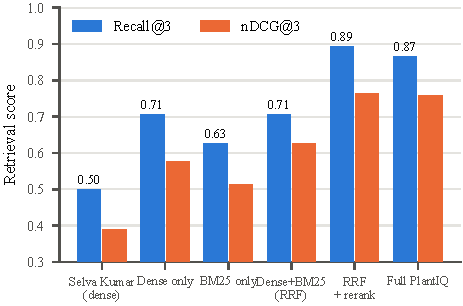
\includegraphics[width=\plantiqfigw]{figures/fig_rag_ablation.pdf}
\caption{Retrieval on 75 questions: the dense baseline and the stages of PlantIQ's retriever.}
\label{fig:ablation}
\end{figure}

Table~\ref{tab:m2} compares the answers. With retrieval, both pipelines stay close to their passages, but PlantIQ's
answers are right more often (0.944 against 0.824, $p=0.02$). Without retrieval the same model answers every question,
and 20\% of its answers give a dose that no document supports, for example pH~7 instead of 9 to 10 for Bordeaux
mixture.

\begin{table}[t]
\caption{Advisory answers, same language model for every system}
\label{tab:m2}
\centering
\footnotesize
\setlength{\tabcolsep}{2.5pt}
\begin{tabular}{@{}lcccc@{}}
\toprule
System & Recall@3 & Correct & Faithful. & \makecell{Unsupported\\doses} \\
\midrule
No retrieval & -- & 0.611 & -- & 20.4\% \\
Dense RAG~\cite{selvakumar2024rag} & 0.500 & 0.824 & 0.990 & 0.0\% \\
PlantIQ & 0.867 & 0.944 & 0.992 & 0.0\% \\
\bottomrule
\end{tabular}
\end{table}

\subsection{Chatbot}
The first chatbot run found three faults, which we fixed before the run in Table~\ref{tab:m3}. The router did not see
the history, so two follow-ups got a wrong value; keyword matching inside words made two Kannada questions look like
weather questions; and offline replies for Kannada users quoted English text. After the fixes, evidence was retrieved
for all ten follow-ups and overall correctness rose from 0.88 to 0.91. Since the fixes were checked on the same
conversations, these figures are optimistic.

PlantIQ behaved as expected in all 43 conversations, against 15 for the baseline ($p<10^{-6}$), and answered 0.91 of
the 29 knowledge questions correctly against 0.38. The baseline has no weather, cannot use a past scan, retrieves
unreadable text for Kannada questions and printed its own instructions when asked to. Its history-aware rewrite did
answer all seven English follow-ups correctly.

\begin{table}[t]
\caption{Chatbot: share of conversations with the expected behaviour and, where a gold answer exists, correctness}
\label{tab:m3}
\centering
\footnotesize
\setlength{\tabcolsep}{2.2pt}
\begin{tabular}{@{}lcccc@{}}
\toprule
 & \multicolumn{2}{c}{Expected} & \multicolumn{2}{c}{Correct} \\
\cmidrule(lr){2-3}\cmidrule(l){4-5}
Group ($n$) & PlantIQ & LangChain & PlantIQ & LangChain \\
\midrule
Follow-up (10) & 1.00 & 0.70 & 0.90 & 0.70 \\
Kannada (10) & 1.00 & 0.00 & 0.85 & 0.00 \\
Photo, scan (8) & 1.00 & 0.38 & 1.00 & 0.44 \\
Weather (8) & 1.00 & 0.00 & -- & -- \\
Greeting (4) & 1.00 & 0.75 & -- & -- \\
Injection (3) & 1.00 & 0.67 & -- & -- \\
\midrule
All (43) & 1.00 & 0.35 & 0.91 & 0.38 \\
\bottomrule
\end{tabular}
\end{table}

\subsection{Speed and Tests}
On the laptop GPU the classifier takes 5.3~ms per image (54.9~ms on the CPU), retrieval about 0.4~s, and a full
advisory about 6~s, most of it spent in the language model. A chat turn without the language model takes a median of
0.22~s. The system has 373 automated tests covering the four modules, security and the user interface.

% =========================================================================================
\section{Limitations}
% =========================================================================================
The classifier knows five classes and was tested on one public dataset of close-up patches from Kenya with only nine
distinct healthy patches; photographs from Karnataka estates are needed, and the choice of backbone should be checked
again on them. The questions and conversations were written by the authors from the same documents the system
searches, and one model both answered and judged. The knowledge base has no readable Phoma document, the infection
risk is a fixed rule rather than a validated model, and speech recognition has not been measured. A field study with
growers is needed to show whether the advice is useful in practice.

% =========================================================================================
\section{Conclusion}
% =========================================================================================
PlantIQ brings leaf diagnosis, grounded and weather-aware advice, a Kannada assistant and a marketplace into one app
that runs on cheap phones. On a leak-free test the classifier is within two points of the best re-implemented
baseline. Hybrid retrieval finds the right passage far more often than a dense pipeline, most of all in Kannada, and
grounding removes the unsupported doses that the same model gives without documents. The chatbot handled all 43 test
conversations, and testing it uncovered three faults that are now fixed.

\section*{Acknowledgment}
The authors thank Prof.\ Deepti C., Department of Computer Science and Engineering, PES University, for guidance
throughout this capstone project, and the Department of Computer Science and Engineering, PES University, for its
support and facilities.

% Column balancing of the reference list; defined only by the two-column wrapper (short.tex).
\providecommand{\plantiqbalancerefs}{}\plantiqbalancerefs
\bibliographystyle{IEEEtran}
\bibliography{references}

\end{document}
